\chapter{Précipitation et solubilité}\label{ch:b1:precipitation}

Une goutte de nitrate d'argent tombe dans de l'eau du robinet et un
nuage blanc apparaît~: du chlorure d'argent, formé à partir des quelques
milligrammes d'ions chlorure que contient chaque litre. L'eau qui
s'infiltre dans le calcaire emporte du carbonate de calcium et le
redépose, à raison d'une fraction de millimètre par an, sous forme de
stalactites. Un calcul rénal est lui aussi un précipité. Chacun de ces
phénomènes est un équilibre entre un solide et ses ions en solution, et
une seule constante, le \omterm{def:b1:precipitation:solubility-product}{produit de solubilité}, dit si le solide se
forme, quelle quantité s'en dissout et comment sa \omterm{def:b1:precipitation:solubility}{solubilité} varie
lorsqu'on ajoute un autre ion ou qu'on change le pH. Grâce à elle, le
chimiste peut séparer des ions les uns des autres en les précipitant
tour à tour --- c'est le principe du traitement des eaux de mine qui
clôt ce chapitre.

\begin{recall}
Le volume scolaire (années 6 et 12) a mesuré la \omterm{def:b1:precipitation:solubility}{solubilité} en grammes
par litre et identifié des ions par les précipités qu'ils donnent. La
constante d'équilibre, le \omterm{def:b1:extent-q-and-k:quotient}{quotient de réaction} $Q$ et les \omterm{def:b1:extent-q-and-k:activity}{activités} (1
pour un solide pur ou pour le solvant, $c/c^\circ$ pour un soluté) ont
été mis en place au \cref{ch:b1:extent-q-and-k}~: une réaction progresse
dans le sens direct tant que $Q < K$. La méthode de la \omterm{def:b1:predominant-reaction:predominant-reaction}{réaction
prépondérante} et l'échelle des $\mathrm{p}K_a$ viennent du
\cref{ch:b1:predominant-reaction}~; on n'écrit pas
$c^\circ = \qty{1}{mol/L}$ dans les quotients.
\end{recall}

\begin{omfigure}
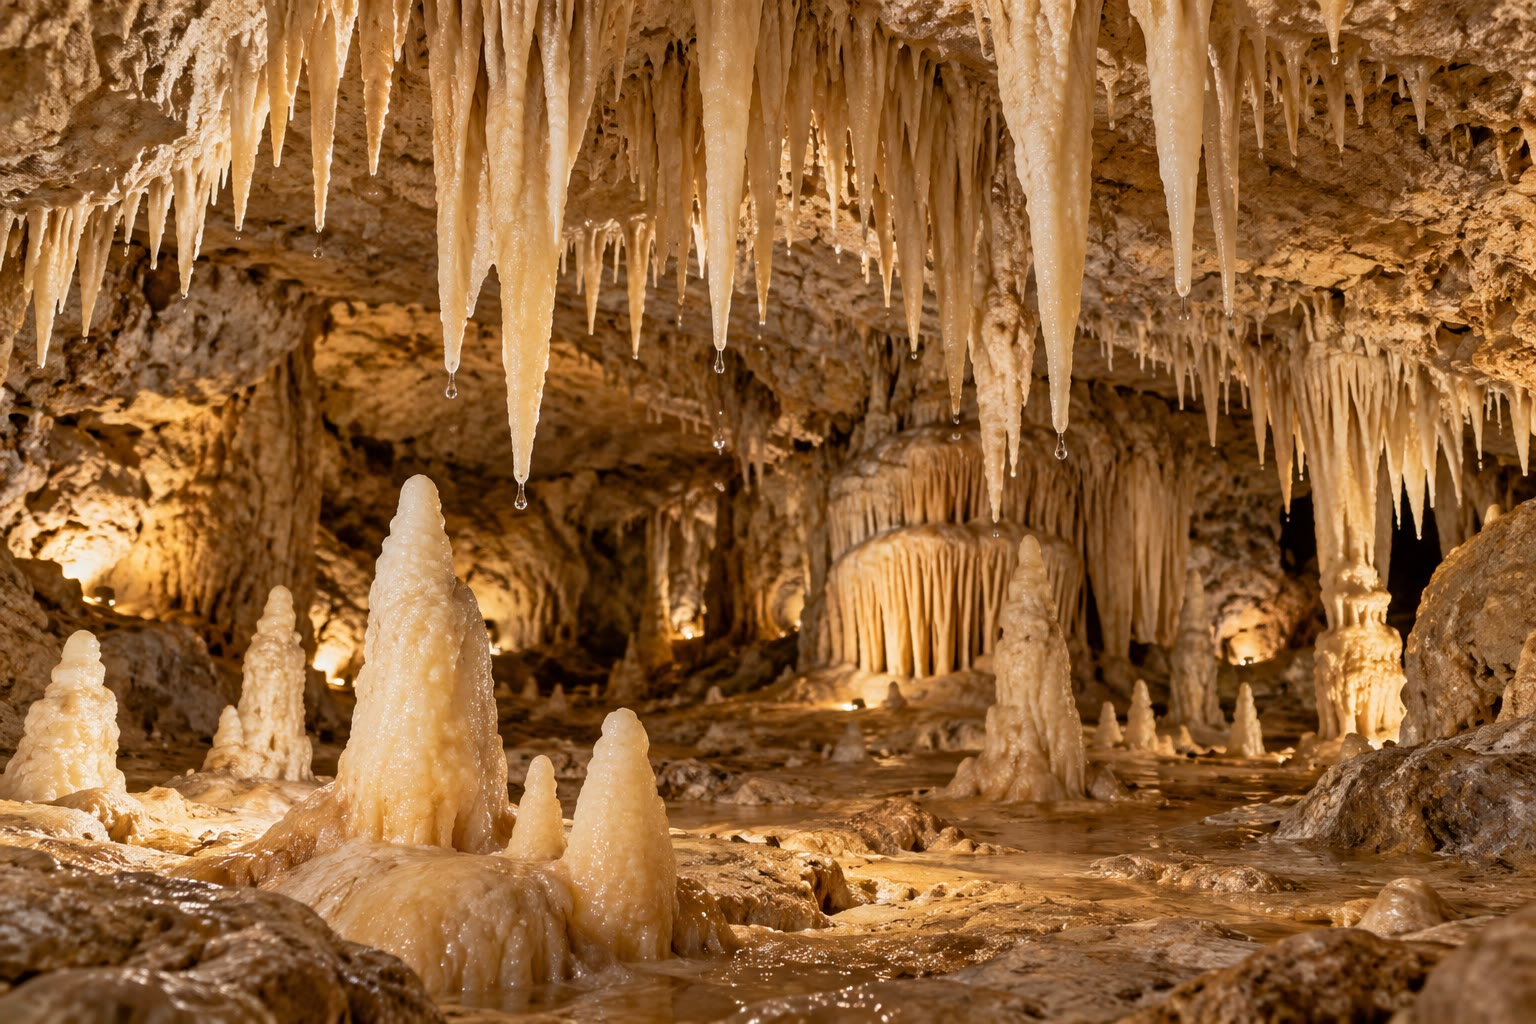
\includegraphics[width=0.62\linewidth]{images/book2/ai/b1-11-cave.jpg}

{\small Stalactites et stalagmites dans une grotte calcaire. L'eau riche
en dioxyde de carbone dissout le carbonate de calcium du sol situé
au-dessus~; dans la grotte, elle perd une partie de son dioxyde de
carbone et le carbonate précipite de nouveau
(\cref{exo:b1:precipitation:10}).}
\end{omfigure}

\section{Le produit de solubilité}\label{sec:b1:precipitation:product}

Un \omterm{def:b1:crystals-metals:crystal}{cristal} de chlorure d'argent plongé dans l'eau cède des ions à la
solution, et la solution en rend au \omterm{def:b1:crystals-metals:crystal}{cristal}. Lorsque les deux vitesses
sont égales, la solution est \emph{saturée}~: sa composition ne varie
plus, bien que des ions continuent de passer dans les deux sens (figure
ci-dessous).

\begin{definition}[Produit de solubilité]\label{def:b1:precipitation:solubility-product}
Le \emph{produit de solubilité}\index{produit de solubilite@produit de solubilité} $K_s$ d'un solide
ionique $\mathrm{M}_a\mathrm{X}_b$ est la constante d'équilibre de sa
dissolution en ses ions,
\[
  \mathrm{M}_a\mathrm{X}_b\mathrm{(s)} \rightleftharpoons a\,\mathrm{M}^{m+}
  + b\,\mathrm{X}^{x-}, \qquad
  K_s = [\mathrm{M}^{m+}]_{\mathrm{eq}}^{\,a}\,[\mathrm{X}^{x-}]_{\mathrm{eq}}^{\,b},
  \qquad \mathrm{p}K_s = -\log K_s ,
\]
l'\omterm{def:b1:extent-q-and-k:activity}{activité} du solide valant 1. Comme toute constante d'équilibre, il ne
dépend que de la température.
\end{definition}

Pour le chlorure d'argent, \ce{AgCl(s) <=> Ag+ + Cl-} et $K_s =
[\ce{Ag+}][\ce{Cl-}] = 10^{-9.75}$~; pour le fluorure de calcium,
\ce{CaF2(s) <=>
Ca^2+ + 2F-} et $K_s = [\ce{Ca^2+}][\ce{F-}]^2 = 10^{-9.84}$~; pour
l'hydroxyde de fer(III), $K_s = [\ce{Fe^3+}][\ce{OH-}]^3 = 10^{-38.55}$.
Le tableau ci-dessous donne les valeurs utilisées dans ce volume. Elles
sont calculées, comme les $\mathrm{p}K_a$ du
\cref{ch:b1:predominant-reaction}, à partir des enthalpies libres
standard de formation tabulées~: $\mathrm{p}K_s = \Delta_r G^\circ/(RT\ln 10)$,
relation établie dans le volume de deuxième année.

\begin{omfigure}
\begin{tikzpicture}[font=\small, >={Stealth}]
  % the crystal: alternating Ag+ (small, grey) and Cl- (large, green)
  \foreach \i in {0,1,2,3,4,5}
    \foreach \j in {0,1,2} {
      \pgfmathtruncatemacro{\pp}{mod(\i+\j,2)}
      \ifnum\pp=0
        \shade[ball color=green!55!black!60] (\i*0.62,\j*0.62) circle (0.29);
      \else
        \shade[ball color=gray!35] (\i*0.62,\j*0.62) circle (0.17);
      \fi }
  \draw[thick, gray] (-0.45,-0.45) rectangle (3.55,1.75);
  \node[below] at (1.55,-0.45) {\ce{AgCl(s)}};
  % ions in solution
  \shade[ball color=gray!35] (1.2,3.0) circle (0.17);
  \node[right] at (1.4,3.0) {\ce{Ag+}};
  \shade[ball color=green!55!black!60] (2.6,2.7) circle (0.29);
  \node[right] at (2.9,2.7) {\ce{Cl-}};
  \shade[ball color=gray!35] (4.4,1.4) circle (0.17);
  \shade[ball color=green!55!black!60] (5.1,2.6) circle (0.29);
  \shade[ball color=gray!35] (-1.0,2.4) circle (0.17);
  \shade[ball color=green!55!black!60] (-0.6,3.3) circle (0.29);
  % arrows: dissolution and precipitation
  \draw[->, thick, omDef] (1.24,1.6) to[bend left=20] node[left, pos=0.6] {dissolution} (1.15,2.78);
  \draw[->, thick, omProp] (2.55,2.38) to[bend left=20] node[right, pos=0.45] {précipitation} (2.45,1.55);
  % the water line
  \draw[blue!50, thick] (-1.6,3.8) -- (5.9,3.8);
  \node[blue!60!black, anchor=east] at (5.9,4.05) {solution saturée};
\end{tikzpicture}

{\small Un \omterm{def:b1:crystals-metals:crystal}{cristal} de chlorure d'argent dans sa solution saturée. Des
ions quittent la surface (dissolution) et d'autres sont captés
(précipitation) à la même vitesse, de sorte que $[\ce{Ag+}][\ce{Cl-}]$
reste égal à $K_s$. Les ions argent sont dessinés plus petits que les
ions chlorure, comme ils le sont réellement.}
\end{omfigure}

\begin{omfigure}
\begin{tabular}{lc@{\qquad}lc}
\hline
solide & $\mathrm{p}K_s$ & solide & $\mathrm{p}K_s$ \\
\hline
\ce{AgCl} & 9.75 & \ce{Ca(OH)2} & 5.33 \\
\ce{AgBr} & 12.27 & \ce{Mg(OH)2} & 11.25 \\
\ce{AgI} & 16.07 & \ce{Fe(OH)2} & 16.31 \\
\ce{Ag2CrO4} & 11.95 & \ce{Zn(OH)2} & 16.38 \\
\ce{BaSO4} & 9.97 & \ce{Fe(OH)3} & 38.55 \\
\ce{CaCO3} (calcite) & 8.30 & \ce{Al(OH)3} (gibbsite) & 34.75 \\
\ce{CaF2} & 9.84 & & \\
\hline
\end{tabular}

\smallskip
{\small \omterm{def:b1:precipitation:solubility-product}{Produits de solubilité} à \qty{25}{\celsius}, calculés à partir
des enthalpies libres standard de formation des solides et des ions en
solution aqueuse. Constantes de formation utilisées dans ce chapitre
(\cref{sec:b1:precipitation:amphoteric})~:
$\log\beta_4 = 14.45$ pour \ce{Zn(OH)4^2-}, 33.52 pour \ce{Al(OH)4-}, et
$\log\beta_1 = 11.82$ pour \ce{FeOH^2+}.}
% ledger: dfg:AgCl_cr, dfg:AgBr_cr, dfg:AgI_cr, dfg:Ag2CrO4_cr, dfg:Ag+_ao, dfg:Cl-_ao, dfg:Br-_ao, dfg:I-_ao, dfg:CrO42-_ao (computed in figdata/bachelor-1/aqueous-constants.py)
% ledger: dfg:BaSO4_cr, dfg:Ba2+_ao, dfg:SO42-_ao, dfg:CaCO3_cr, dfg:CO32-_ao, dfg:CaF2_cr, dfg:Ca2+_ao, dfg:F-_ao (computed, same script)
% ledger: dfg:Ca_OH2_cr, dfg:Mg_OH2_cr, dfg:Mg2+_ao, dfg:Fe_OH2_cr, dfg:Fe2+_ao, dfg:Zn_OH2_cr, dfg:Zn2+_ao, dfg:Fe_OH3_cr, dfg:Fe3+_ao, dfg:Al2O3.3H2O_cr, dfg:Al3+_ao, dfg:OH-_ao (computed, same script)
% ledger: dfg:Zn_OH42-_ao, dfg:Al_OH4-_ao, dfg:FeOH2+_ao (formation constants, same script)
\end{omfigure}

\begin{proposition}[Condition de précipitation]\label{prop:b1:precipitation:precipitation-condition}
Soit une solution contenant les ions d'un solide
$\mathrm{M}_a\mathrm{X}_b$, de \omterm{def:b1:extent-q-and-k:quotient}{quotient de réaction}
$Q_s = [\mathrm{M}^{m+}]^a[\mathrm{X}^{x-}]^b$ pour la dissolution.
\begin{itemize}
  \item Si $Q_s < K_s$, le solide ne peut pas être présent à
        l'équilibre~: la solution n'est pas saturée et tout solide ajouté
        se dissout, entièrement s'il n'y en a pas trop.
  \item Si $Q_s > K_s$, le solide précipite jusqu'à ce que $Q_s = K_s$.
  \item Le solide et la solution ne coexistent à l'équilibre que si
        $Q_s = K_s$.
\end{itemize}
\end{proposition}

\begin{proof}
D'après le \cref{ch:b1:extent-q-and-k}, la dissolution progresse tant
que $Q_s < K_s$ et régresse (précipitation) tant que $Q_s > K_s$. Pendant
que la dissolution progresse, $Q_s$ augmente. Si le solide est épuisé
avant que $Q_s$ atteigne $K_s$, l'évolution s'arrête sans solide
restant~: une réaction faisant intervenir une \omterm{def:b1:extent-q-and-k:system}{phase} condensée pure peut
s'arrêter avant l'équilibre parce que la quantité de cette \omterm{def:b1:extent-q-and-k:system}{phase} ne peut
pas devenir négative. Si $Q_s > K_s$, la précipitation diminue les deux
concentrations ioniques et $Q_s$ décroît jusqu'à égaler $K_s$, ce qui
est toujours possible, puisque les ions sont présents.
\end{proof}

Ce dernier point distingue un solide d'une espèce dissoute. Une espèce
acido-basique est présente à tout pH, si peu que ce soit~; un solide
est présent ou absent. C'est pourquoi son diagramme sera un diagramme
d'\emph{existence}, et non de prédominance
(\cref{sec:b1:precipitation:domains}).

\begin{example}[Mélanger deux solutions]\label{ex:b1:precipitation:mixing}
On mélange \qty{10.0}{mL} de nitrate d'argent à \qty{2.0e-4}{mol/L} et
\qty{10.0}{mL} de chlorure de sodium à \qty{2.0e-4}{mol/L}. Juste après
le mélange, avant toute réaction, $[\ce{Ag+}] = [\ce{Cl-}] = \qty{1.0e-4}{mol/L}$
et $Q_s = 10^{-8.0} > K_s = 10^{-9.75}$~: le chlorure d'argent
précipite. Avec les deux solutions à \qty{2.0e-6}{mol/L}, $Q_s = 10^{-12.0} < K_s$ et le
mélange reste limpide. Le nitrate d'argent est un test sensible des ions
chlorure, mais pas infiniment sensible.
\end{example}

\begin{inthelab}[Le test des chlorures]
En travaux pratiques, on ajoute quelques gouttes de solution de nitrate
d'argent à l'échantillon, préalablement acidifié par de l'acide nitrique
dilué. L'acide transforme les ions carbonate et hydroxyde en dioxyde de
carbone et en eau, qui sinon précipiteraient eux aussi avec les ions
argent. Un précipité blanc qui noircit à la lumière est du chlorure
d'argent~; les bromures donnent un précipité crème et les iodures un
précipité jaune (photographie ci-dessous). Le nitrate d'argent tache la
peau en noir~: on porte des gants et des lunettes.
\end{inthelab}

\begin{omfigure}
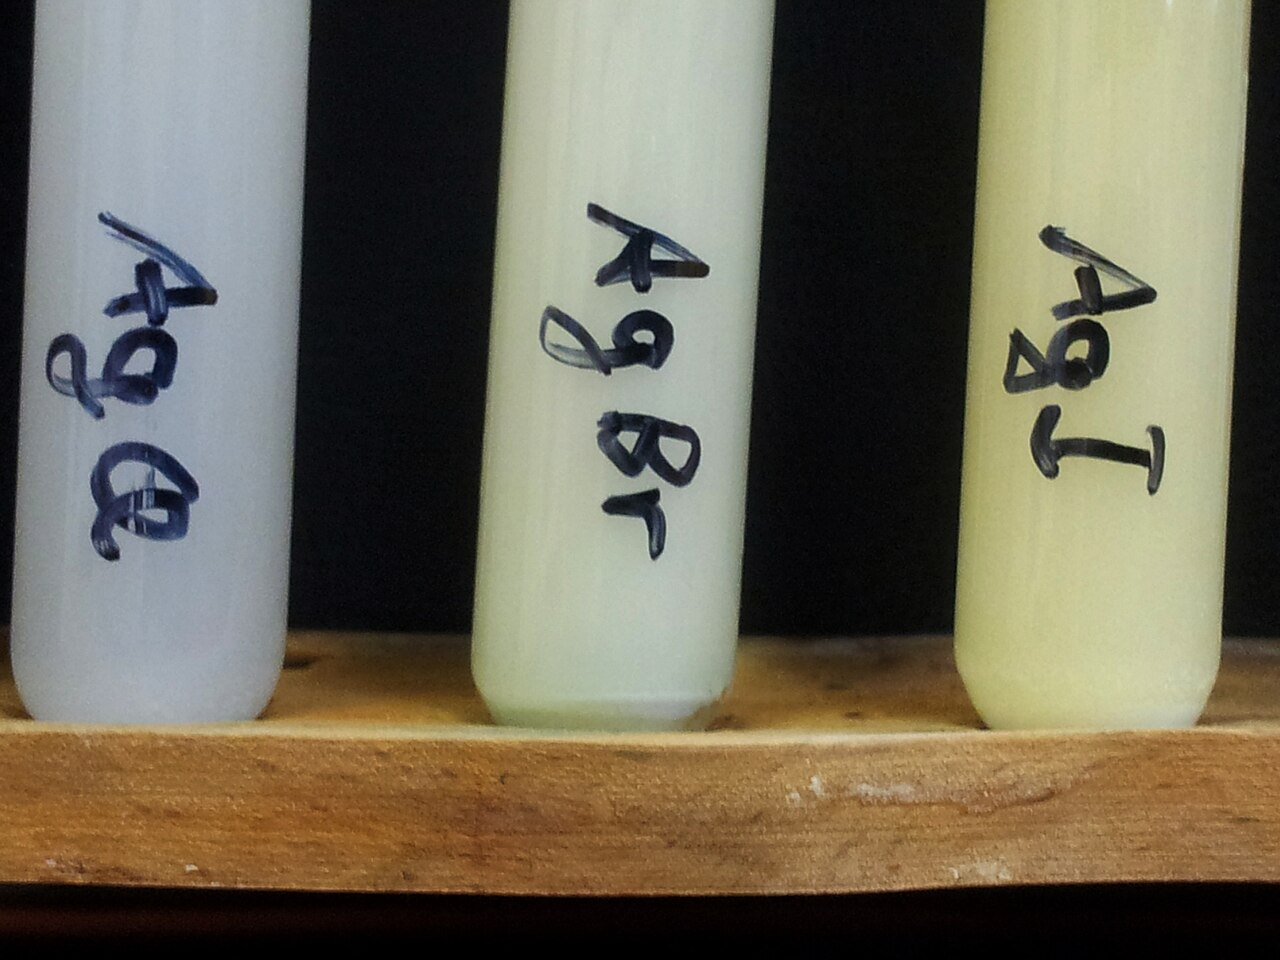
\includegraphics[width=0.6\linewidth]{images/book2/silver-halides.jpg}

{\small Précipités de chlorure d'argent (blanc), de bromure d'argent
(crème) et d'iodure d'argent (jaune pâle). Photographie Rrausch1974,
CC BY-SA 3.0, Wikimedia Commons.}
\end{omfigure}

\section{Solubilité}

\begin{definition}[Solubilité]\label{def:b1:precipitation:solubility}
La \emph{solubilité}\index{solubilite@solubilité} $s$ d'un solide dans une solution donnée
est la quantité de solide qui se dissout dans un litre de cette
solution jusqu'à saturation (en \unit{mol/L})~; multipliée par la masse
molaire, c'est la solubilité massique, en \unit{g/L}. Elle dépend de la
température et de la composition de la solution.
\end{definition}

\begin{proposition}[Solubilité et produit de solubilité]\label{prop:b1:precipitation:s-of-ks}
Dans l'eau pure, si les ions ne participent à aucune autre réaction,
\[
  \mathrm{MX}:\ s = \sqrt{K_s}, \qquad
  \mathrm{MX_2}\ \text{ou}\ \mathrm{M_2X}:\ s = \left(\frac{K_s}{4}\right)^{1/3},
  \qquad
  \mathrm{M}_a\mathrm{X}_b:\ s = \left(\frac{K_s}{a^a b^b}\right)^{1/(a+b)} .
\]
\end{proposition}

\begin{proof}
Lorsque $s$ mol de solide se dissolvent par litre, $[\mathrm{M}^{m+}] = as$ et
$[\mathrm{X}^{x-}] = bs$, donc à saturation $K_s = (as)^a(bs)^b =
a^a b^b s^{a+b}$. Pour MX, $a = b = 1$~; pour \ce{MX2}, $1^1 2^2 = 4$,
et de même pour \ce{M2X}.
\end{proof}

\begin{example}[Chlorure d'argent et chromate d'argent]\label{ex:b1:precipitation:agcl-ag2cro4}
Chlorure d'argent~: $s = 10^{-9.75/2} = \qty{1.3e-5}{mol/L}$, soit
\qty{1.9}{mg/L} avec $M = \qty{143.4}{g/mol}$. Chromate d'argent
\ce{Ag2CrO4} ($\mathrm{p}K_s = 11.95$)~: $s = (10^{-11.95}/4)^{1/3} =
\qty{6.6e-5}{mol/L}$. Le chromate a le plus petit $K_s$ et pourtant il
est cinq fois plus soluble. On ne peut comparer directement les \omterm{def:b1:precipitation:solubility-product}{produits
de solubilité} qu'entre solides de même type de formule.
\end{example}

\begin{remark}
Ces formules supposent que les ions sont libres. Dans l'eau pure, l'ion
chromate est une \omterm{def:b1:predominant-reaction:strong-acid}{base faible} et l'ion argent n'est complexé par rien, si
bien que le résultat pour le chromate d'argent est à peu près exact~;
pour un carbonate, un sulfure ou un hydroxyde, les propriétés basiques
de l'anion comptent et il faut la section suivante. À force ionique
élevée, les \omterm{def:b1:extent-q-and-k:activity}{activités} s'écartent aussi des concentrations, correction
laissée au volume de deuxième année.
\end{remark}

\section{Effet d'ion commun et effet du pH}

\begin{definition}[Effet d'ion commun]\label{def:b1:precipitation:common-ion}
L'\emph{effet d'ion commun}\index{effet d'ion commun} est la diminution
de la \omterm{def:b1:precipitation:solubility}{solubilité} d'un solide dans une solution qui contient déjà l'un de
ses ions.
\end{definition}

\begin{proposition}[Solubilité en présence d'un ion commun]\label{prop:b1:precipitation:common-ion}
Soit MX se dissolvant dans une solution où l'on a déjà
$[\mathrm{X}^-] = c$, avec
$c \gg \sqrt{K_s}$. Alors $s \approx K_s/c$, bien plus faible que dans
l'eau pure. Pour \ce{MX2} dans une solution contenant \ce{M^2+} à la
concentration $c$,
$s \approx \frac12\sqrt{K_s/c}$.
\end{proposition}

\begin{proof}
À saturation, $[\mathrm{M}^+] = s$ et $[\mathrm{X}^-] = c + s$, donc
$s(c + s) = K_s$. Si $s \ll c$, $s = K_s/c$~; l'hypothèse est vérifiée
puisque $K_s/c \ll c$ lorsque $c^2 \gg K_s$. Pour \ce{MX2},
$[\ce{X-}] = 2s$ et
$[\mathrm{M}^{2+}] = c + s \approx c$, donc $c\,(2s)^2 = K_s$.
\end{proof}

Chlorure d'argent dans une solution de chlorure de sodium à
\qty{0.10}{mol/L}~: $s = 10^{-9.75}/0.10
= \qty{1.8e-9}{mol/L}$, sept mille fois moins que dans l'eau. C'est
pourquoi l'on lave un précipité avec une solution diluée d'un ion
commun plutôt qu'avec de l'eau pure~: il s'y dissout moins.

Lorsque l'anion du solide est une base, un acide l'extrait de
l'équilibre de dissolution et la \omterm{def:b1:precipitation:solubility}{solubilité} augmente. Pour le carbonate
de calcium en milieu acide,
\[
  \ce{CaCO3(s) + H3O+ <=> Ca^2+ + HCO3- + H2O}, \qquad
  K = \frac{K_s}{K_{a2}} = 10^{-8.30 + 10.33} = 10^{2.03} ,
\]
réaction favorisée~: le vinaigre ou l'acide chlorhydrique dissolvent le
calcaire, et le dioxyde de carbone formé par la réaction ultérieure de
\ce{HCO3-} produit l'effervescence bien connue.
% ledger: dfg:HCO3-_ao (pKa2 of carbonic acid, ch. 10)

\begin{proposition}[Solubilité d'un hydroxyde en fonction du pH]\label{prop:b1:precipitation:hydroxide-ph}
Dans une solution tamponnée à un pH donné, la concentration de \ce{M^{n+}}
en équilibre avec l'hydroxyde \ce{M(OH)_n} vérifie
\[
  \log[\mathrm{M}^{n+}] = -\mathrm{p}K_s + n\,(\mathrm{p}K_e - \mathrm{pH}) ,
\]
droite de pente $-n$ en fonction du pH. Si l'ion ne forme aucun
complexe, c'est la \omterm{def:b1:precipitation:solubility}{solubilité} de l'hydroxyde.
\end{proposition}

\begin{proof}
$K_s = [\mathrm{M}^{n+}][\ce{OH-}]^n$ et $[\ce{OH-}] = K_e/[\ce{H3O+}]$,
donc $\log[\mathrm{M}^{n+}] = \log K_s - n\log[\ce{OH-}] = -\mathrm{p}K_s -
n(\mathrm{pH} - \mathrm{p}K_e)$.
\end{proof}

Chaque unité de pH divise par mille la \omterm{def:b1:precipitation:solubility}{solubilité} de l'hydroxyde de
fer(III) et par cent celle de l'hydroxyde de zinc. On précipite les
hydroxydes, et on les redissout, en changeant le pH.

\begin{example}[Dissoudre le carbonate de calcium par le dioxyde de carbone]\label{ex:b1:precipitation:cave}
Une eau qui contient du dioxyde de carbone dissous dissout la calcite~:
\[
  \ce{CaCO3(s) + CO2(aq) + H2O <=> Ca^2+ + 2HCO3-}, \qquad
  K = \frac{K_s K_{a1}}{K_{a2}} = 10^{-8.30 - 6.37 + 10.33} = 10^{-4.34} ,
\]
la constante s'obtenant en additionnant la dissolution du carbonate, la
première acidité du dioxyde de carbone et l'inverse de la seconde. Plus
il y a de dioxyde de carbone, plus le carbonate de calcium se dissout.
L'air du sol est en général bien plus riche en dioxyde de carbone que
l'air d'une grotte~; l'eau qui a traversé le sol et atteint la voûte de
la grotte perd du dioxyde de carbone, et la calcite se dépose
(\cref{exo:b1:precipitation:10}).
\end{example}

\section{Domaines d'existence et précipitation sélective}\label{sec:b1:precipitation:domains}

\begin{definition}[Domaine d'existence]\label{def:b1:precipitation:existence-domain}
Pour un solide et une concentration totale $c$ donnée de l'un de ses
ions, le \emph{domaine d'existence}\index{domaine d'existence} du solide
est l'intervalle de la variable (pX, pM ou pH) sur lequel le solide est
présent à l'équilibre. Sa frontière est la valeur pour laquelle apparaît
le premier grain de solide, lorsque $Q_s = K_s$ avec l'ion encore à la
concentration $c$.
\end{definition}

\begin{method}[Tracer un diagramme d'existence]\label{met:b1:precipitation:existence-domain}
\begin{enumerate}
  \item Fixer la concentration totale $c$ de l'ion qui n'est pas porté
        sur l'axe (par exemple $[\ce{Ag+}]_{\mathrm{tot}} = c$ sur un axe
        de pCl).
  \item Écrire $K_s$ au début de la précipitation, l'ion étant encore à
        la concentration $c$, et résoudre en la variable portée sur l'axe.
  \item Le solide existe du côté où l'autre ion est concentré~: petit pCl
        (beaucoup de chlorure), petit pAg, ou pH élevé pour un hydroxyde.
  \item Ne pas tracer de domaine pour l'ion lui-même~: il est présent
        partout, à la concentration $c$ hors du domaine du solide et à une
        concentration inférieure à $c$ à l'intérieur.
\end{enumerate}
\end{method}

Pour le chlorure d'argent avec $c = [\ce{Ag+}]_{\mathrm{tot}} = 10^{-2}$~:
la précipitation commence quand $[\ce{Cl-}] = K_s/c = 10^{-7.75}$, et le
solide existe donc pour $\mathrm{pCl} < 7.75$. Pour l'iodure d'argent, la
frontière est à $\mathrm{pI} = 16.07 - 2 = 14.07$, comme le montre la
figure ci-dessous.

\begin{omfigure}
\begin{tikzpicture}[font=\small, >={Stealth}, x=0.62cm]
  \fill[omDef!18] (0,0.12) rectangle (7.75,0.6);
  \draw[->, thick] (0,0) -- (17.2,0) node[right] {pCl ou pI};
  \foreach \x in {0,2,4,6,8,10,12,14,16}
    \draw (\x,0.08) -- (\x,-0.08) node[below] {\x};
  \draw[omDef, thick] (7.75,-0.5) -- (7.75,0.9);
  \node[omDef] at (3.9,0.36) {\ce{AgCl(s)} existe};
  \node[omDef, above] at (7.75,0.9) {7.75};
  \node[anchor=west] at (8.0,0.36) {pas de solide~: \ce{Ag+} à $10^{-2}$ mol/L};
  % AgI below
  \begin{scope}[yshift=-1.9cm]
  \fill[omProp!20] (0,0.12) rectangle (14.07,0.6);
  \draw[->, thick] (0,0) -- (17.2,0);
  \foreach \x in {0,2,4,6,8,10,12,14,16}
    \draw (\x,0.08) -- (\x,-0.08) node[below] {\x};
  \draw[omProp, thick] (14.07,-0.5) -- (14.07,0.9);
  \node[omProp] at (7.0,0.36) {\ce{AgI(s)} existe};
  \node[omProp, above] at (14.07,0.9) {14.07};
  \end{scope}
\end{tikzpicture}

{\small \omterm{def:b1:precipitation:existence-domain}{Domaines d'existence} du chlorure d'argent (sur un axe de pCl, en
haut) et de l'iodure d'argent (sur un axe de pI, en bas) pour une
concentration totale en argent de \qty{1.0e-2}{mol/L}. L'iodure
précipite l'argent à des concentrations un million de fois plus faibles
que le chlorure.}
\end{omfigure}

\begin{method}[Précipitation sélective]\label{met:b1:precipitation:selective}
Pour séparer deux ions qui précipitent avec le même réactif~:
\begin{enumerate}
  \item calculer, pour chaque ion à sa concentration, la concentration de
        réactif (ou le pH) à laquelle son solide commence à se former~;
        la plus faible précipite en premier~;
  \item calculer la concentration du premier ion restant en solution
        lorsque le second commence à précipiter~;
  \item la séparation est acceptable si cette concentration est une
        fraction assez petite de la concentration initiale ---
        typiquement \qty{0.1}{\percent} ---, et l'on arrête alors l'ajout
        de réactif entre les deux seuils.
\end{enumerate}
\end{method}

\begin{example}[Iodure et chlorure]\label{ex:b1:precipitation:i-cl}
Une solution contient des ions iodure et chlorure, tous deux à
\qty{1.0e-2}{mol/L}~; on y ajoute du nitrate d'argent goutte à goutte,
sans dilution. L'iodure d'argent commence à se former pour
$[\ce{Ag+}] = 10^{-16.07 + 2} =
10^{-14.07}$, le chlorure d'argent pour $10^{-9.75 + 2} = 10^{-7.75}$~:
l'iodure précipite en premier. Quand le chlorure d'argent apparaît,
$[\ce{I-}] = 10^{-16.07}/10^{-7.75} = 10^{-8.32} = \qty{4.8e-9}{mol/L}$,
soit une fraction $5 \times 10^{-7}$ de l'iodure~: la séparation est
complète.
\end{example}

On sépare de même les hydroxydes, avec le pH pour variable. Le
graphique ci-dessous indique, pour six ions à \qty{0.010}{mol/L}, le pH
où l'hydroxyde apparaît et le pH où \qty{99.9}{\percent} de l'ion a
précipité. Le fer(III) et l'aluminium sont éliminés en milieu acide, le
zinc et le fer(II) vers la neutralité, le magnésium vers pH 10 et le
calcium seulement en milieu très basique.

\begin{omfigure}
\begin{tikzpicture}
\begin{axis}[
  width=0.82\linewidth, height=5.4cm, xmin=0, xmax=14, ymin=0.4, ymax=6.6,
  axis x line=bottom, axis y line=left, xlabel={pH},
  xtick={0,2,4,6,8,10,12,14}, ytick={1,2,3,4,5,6},
  yticklabels={\ce{Fe^3+}, \ce{Al^3+}, \ce{Zn^2+}, \ce{Fe^2+}, \ce{Mg^2+}, \ce{Ca^2+}},
  y dir=reverse, axis line style={-},
  tick label style={font=\small}, label style={font=\small}]
\addplot[draw=none, omDef!35,
  error bars/.cd, x dir=plus, x explicit,
  error bar style={line width=7pt, omDef!35}, error mark=none]
  table[x=start, y=row, x error expr=14-\thisrow{start}] {figdata/out/bachelor-1-solubility-ph-thresholds.dat};
\addplot[draw=none, omDef,
  error bars/.cd, x dir=plus, x explicit,
  error bar style={line width=7pt, omDef}, error mark=none]
  table[x=start, y=row, x error expr=\thisrow{end}-\thisrow{start}] {figdata/out/bachelor-1-solubility-ph-thresholds.dat};
\end{axis}
\end{tikzpicture}

{\small Précipitation des hydroxydes à partir de solutions à
\qty{0.010}{mol/L} de chaque ion. La barre foncée va du premier grain
d'hydroxyde au pH où \qty{99.9}{\percent} de l'ion a précipité (une
unité de pH de large pour un ion trivalent, une et demie pour un ion
divalent)~; la barre claire est le reste du \omterm{def:b1:precipitation:existence-domain}{domaine d'existence} de
l'hydroxyde. La redissolution amphotère des hydroxydes de zinc et
d'aluminium à pH élevé (\cref{sec:b1:precipitation:amphoteric}) n'est
pas représentée.}
\end{omfigure}

\section{Hydroxydes amphotères}\label{sec:b1:precipitation:amphoteric}

On ajoute goutte à goutte de l'hydroxyde de sodium à une solution de
sulfate de zinc~: un précipité blanc d'hydroxyde de zinc se forme, puis,
en excès d'hydroxyde, il se redissout. L'hydroxyde d'aluminium fait de
même~; les hydroxydes de fer(III) et de magnésium, non.

\begin{definition}[Hydroxyde amphotère]\label{def:b1:precipitation:amphoteric-hydroxide}
Un hydroxyde est un \emph{hydroxyde amphotère}\index{hydroxyde amphotere@hydroxyde amphotère}
s'il se dissout à la fois en milieu acide, sous forme de cation, et dans
un excès de base, sous forme d'anion complexe hydroxo~:
\[
  \ce{Zn(OH)2(s) + 2H3O+ -> Zn^2+ + 4H2O}, \qquad
  \ce{Zn(OH)2(s) + 2OH- -> Zn(OH)4^2-} .
\]
\end{definition}

L'anion complexe \ce{Zn(OH)4^2-} (ion tétrahydroxozincate) est
caractérisé par sa constante de formation
$\beta_4 = [\ce{Zn(OH)4^2-}]/([\ce{Zn^2+}][\ce{OH-}]^4)
= 10^{14.45}$~; les complexes et leurs constantes font l'objet du
\cref{ch:b1:complexation}.

\begin{proposition}[Solubilité d'un hydroxyde amphotère]\label{prop:b1:precipitation:amphoteric}
Si le zinc n'est en solution que sous les formes \ce{Zn^2+} et
\ce{Zn(OH)4^2-}, la \omterm{def:b1:precipitation:solubility}{solubilité} de l'hydroxyde de zinc vaut
\[
  s = [\ce{Zn^2+}] + [\ce{Zn(OH)4^2-}] = \frac{K_s}{[\ce{OH-}]^2} + K\,[\ce{OH-}]^2,
  \qquad K = \beta_4 K_s = 10^{-1.93} .
\]
En $\log s$ en fonction du pH, elle suit une droite de pente $-2$ à bas
pH et une droite de pente $+2$ à pH élevé. Elle est minimale pour
$[\ce{OH-}]^4 = K_s/K = 1/\beta_4$, c'est-à-dire à $\mathrm{pH} =
\mathrm{p}K_e - \frac14\log\beta_4$, où $s_{\min} = 2\sqrt{K_s K}$.
\end{proposition}

\begin{proof}
À saturation, on a $[\ce{Zn^2+}] = K_s/[\ce{OH-}]^2$, tandis que la
concentration de l'ion zincate vaut
$[\ce{Zn(OH)4^2-}] = \beta_4[\ce{Zn^2+}][\ce{OH-}]^4 = \beta_4 K_s
[\ce{OH-}]^2$. Avec $w = [\ce{OH-}]^2$, $s(w) = K_s/w + Kw$ a pour dérivée
$-K_s/w^2 + K$, nulle en $w = \sqrt{K_s/K}$, où $s = 2\sqrt{K_s K}$. À
bas pH, le premier terme domine et $\log s = \log K_s - 2\log[\ce{OH-}]$
(pente $-2$ en pH)~; à pH élevé, c'est le second,
$\log s = \log K + 2\log[\ce{OH-}]$ (pente $+2$).
\end{proof}

Avec les valeurs ci-dessus, le minimum se situe à $\mathrm{pH} = 14.00 - 14.45/4
= 10.39$ et $s_{\min} = 2 \times 10^{-(16.38 + 1.93)/2} =
\qty{1.4e-9}{mol/L}$
(figure ci-dessous). Le minimum réel est bien plus élevé~: le zinc forme
aussi \ce{ZnOH+}, \ce{Zn(OH)3-} et surtout une espèce dissoute non
chargée, \ce{Zn(OH)2(aq)}, dont la concentration en équilibre avec le
solide ne dépend pas du pH. Le calcul complet, avec les mêmes tables,
place le plancher vers
$10^{-5.6}$~mol/L. Un modèle à deux espèces donne les pentes et l'ordre
des seuils~; près du minimum, toutes les espèces comptent.

\begin{omfigure}
\begin{tikzpicture}
\begin{axis}[name=zn,
  width=0.46\linewidth, height=5.6cm, xmin=6, xmax=14, ymin=-10, ymax=0,
  axis x line=bottom, axis y line=left, xlabel={pH}, ylabel={$\log s$},
  xtick={6,8,10,12,14}, ytick={-10,-8,-6,-4,-2,0},
  tick label style={font=\small}, label style={font=\small}]
\addplot[omProp, dashed, thick] table[x=pH, y=full] {figdata/out/bachelor-1-solubility-ph-zinc.dat};
\addplot[omDef, very thick] table[x=pH, y=model] {figdata/out/bachelor-1-solubility-ph-zinc.dat};
\node[font=\small, anchor=west] at (axis cs:7.0,-1.0) {\ce{Zn^2+}};
\node[font=\small, anchor=east] at (axis cs:13.8,-1.1) {\ce{Zn(OH)4^2-}};
\node[font=\small, omProp, anchor=south] at (axis cs:10.4,-5.5) {toutes les espèces};
\node[font=\small, anchor=north] at (axis cs:10.2,-0.4) {zinc};
\end{axis}
\begin{axis}[at={(zn.east)}, anchor=west, xshift=1.8cm,
  width=0.46\linewidth, height=5.6cm, xmin=2, xmax=14, ymin=-10, ymax=0,
  axis x line=bottom, axis y line=left, xlabel={pH}, ylabel={$\log s$},
  xtick={2,4,6,8,10,12,14}, ytick={-10,-8,-6,-4,-2,0},
  tick label style={font=\small}, label style={font=\small}]
\addplot[omDef, very thick] table[x=pH, y=model] {figdata/out/bachelor-1-solubility-ph-aluminium.dat};
\node[font=\small, anchor=west] at (axis cs:3.4,-0.8) {\ce{Al^3+}};
\node[font=\small, anchor=east] at (axis cs:13.8,-0.6) {\ce{Al(OH)4-}};
\node[font=\small, anchor=north] at (axis cs:8.6,-0.4) {aluminium};
\end{axis}
\end{tikzpicture}

{\small \omterm{def:b1:precipitation:solubility}{Solubilité} de l'hydroxyde de zinc (à gauche) et de l'hydroxyde
d'aluminium, la gibbsite (à droite), en fonction du pH, modèle à deux
espèces (traits pleins)~: pentes $-2$ et $+2$ pour le zinc, $-3$ et $+1$
pour l'aluminium. Pour le zinc, la courbe en tirets inclut toutes les
espèces hydroxo, l'espèce non chargée \ce{Zn(OH)2(aq)} imposant un
plancher.}
\end{omfigure}

Pour l'aluminium, l'hydroxyde est \ce{Al(OH)3} et le complexe
\ce{Al(OH)4-}, donc $\ce{Al(OH)3(s) + OH- <=> Al(OH)4-}$ avec $K = \beta_4 K_s = 10^{33.52
- 34.75} = 10^{-1.23}$ et les pentes $-3$ et $+1$. La différence entre
l'aluminium et le fer(III) --- l'un amphotère, l'autre non --- sert dans
l'industrie à les séparer~: la soude chaude dissout l'aluminium de la
bauxite et laisse les oxydes de fer (\cref{exo:b1:precipitation:12}).

\section{Exercices}

\begin{exercise}[$\star$]\label{exo:b1:precipitation:1}
Écrire l'équation de dissolution et l'expression de $K_s$ pour
\ce{BaSO4}, \ce{CaF2}, \ce{Ag2CrO4} et \ce{Fe(OH)3}. Donner $K_s$ en
puissances de dix à partir du tableau de la
\cref{sec:b1:precipitation:product}, ainsi que le $\mathrm{p}K_s$ d'un
solide de $K_s = \num{2.0e-13}$.
\end{exercise}

\begin{exercise}[$\star$]\label{exo:b1:precipitation:2}
Calculer la \omterm{def:b1:precipitation:solubility}{solubilité} du bromure d'argent dans l'eau pure en
\unit{mol/L} et en \unit{mg/L} ($M = \qty{187.8}{g/mol}$).
\end{exercise}

\begin{exercise}[$\star$]\label{exo:b1:precipitation:3}
On mélange \qty{50}{mL} de chlorure de baryum à \qty{2.0e-3}{mol/L} et
\qty{50}{mL} de sulfate de sodium à \qty{2.0e-4}{mol/L}. Le sulfate de
baryum précipite-t-il~? Même question avec le sulfate de sodium à
\qty{2.0e-7}{mol/L}.
\end{exercise}

\begin{exercise}[$\star$]\label{exo:b1:precipitation:4}
Calculer la \omterm{def:b1:precipitation:solubility}{solubilité} du sulfate de baryum dans l'eau pure, puis dans
une solution de sulfate de sodium à \qty{0.010}{mol/L}. De quel facteur
a-t-elle varié~?
\end{exercise}

\begin{exercise}[$\star\star$]\label{exo:b1:precipitation:5}
Calculer la \omterm{def:b1:precipitation:solubility}{solubilité} du fluorure de calcium dans l'eau pure
(\unit{mol/L} et \unit{mg/L}, $M = \qty{78.1}{g/mol}$), puis dans une
solution de chlorure de calcium à \qty{0.10}{mol/L}. Vérifier
l'approximation faite.
\end{exercise}

\begin{exercise}[$\star\star$]\label{exo:b1:precipitation:6}
Une solution contient des ions magnésium à \qty{0.050}{mol/L}. À quel pH
l'hydroxyde de magnésium commence-t-il à précipiter~? À quel pH
\qty{99}{\percent} du magnésium a-t-il précipité~? Tracer le \omterm{def:b1:precipitation:existence-domain}{domaine
d'existence} de \ce{Mg(OH)2} sur un axe de pH.
\end{exercise}

\begin{exercise}[$\star\star$]\label{exo:b1:precipitation:7}
Une solution contient des ions bromure et chlorure, tous deux à
\qty{1.0e-2}{mol/L}. On ajoute du nitrate d'argent sans dilution. Quel
précipité apparaît en premier~? Quelle fraction du premier ion reste en
solution quand le second solide apparaît~? La séparation est-elle
acceptable~?
\end{exercise}

\begin{exercise}[$\star\star$]\label{exo:b1:precipitation:8}
Le titrage de Mohr des chlorures par les ions argent utilise les ions
chromate comme indicateur~: le chromate d'argent, rouge, ne doit
apparaître qu'une fois presque tout le chlorure précipité. Le chlorure
est à \qty{0.050}{mol/L} et le chromate à \qty{5.0e-3}{mol/L}~; on
néglige la dilution. Calculer $[\ce{Ag+}]$ quand le chromate d'argent
commence à se former, et la fraction de chlorure encore en solution à
cet instant.
\end{exercise}

\begin{exercise}[$\star\star$]\label{exo:b1:precipitation:9}
On agite du carbonate de calcium avec une solution maintenue à pH 8.30
par un tampon, où l'hydrogénocarbonate est de loin l'espèce carbonatée
majoritaire. Montrer que
$[\ce{Ca^2+}][\ce{HCO3-}] = K_s\,10^{\mathrm{p}K_{a2} - \mathrm{pH}}$, et
calculer la \omterm{def:b1:precipitation:solubility}{solubilité}, en admettant que tout le carbonate dissous
reste sous la forme \ce{HCO3-} ($\mathrm{p}K_{a2} = 10.33$).
\end{exercise}

\begin{exercise}[$\star\star\star$]\label{exo:b1:precipitation:10}
Grottes calcaires. La \omterm{def:b1:precipitation:solubility}{solubilité} du dioxyde de carbone suit
\ce{CO2(g) <=> CO2(aq)} avec $\log K_H = -1.47$ ($K_H =
[\ce{CO2(aq)}]/p(\ce{CO2})$, pression en bar).
\begin{enumerate}
  \item Combiner $K_H$ avec la constante de
        l'\cref{ex:b1:precipitation:cave} pour obtenir la constante de
        \ce{CaCO3(s) + CO2(g) + H2O <=> Ca^2+ + 2HCO3-}.
  \item Montrer que la \omterm{def:b1:precipitation:solubility}{solubilité} de la calcite vaut $s = (K'p/4)^{1/3}$
        et la calculer pour une eau en équilibre avec l'air du sol, à
        $p(\ce{CO2}) = \qty{0.010}{bar}$, puis avec l'air extérieur,
        \qty{4.26e-4}{bar}. Donner les deux en \unit{mg/L} de \ce{CaCO3}
        ($M = \qty{100.1}{g/mol}$).
  \item Expliquer la croissance d'une stalactite.
\end{enumerate}
\end{exercise}

\begin{exercise}[$\star\star\star$]\label{exo:b1:precipitation:11}
Une solution de zinc à \qty{1.0e-2}{mol/L} est portée à des pH
croissants, le zinc n'étant présent que sous les formes \ce{Zn^2+} et
\ce{Zn(OH)4^2-}.
\begin{enumerate}
  \item Entre quelles valeurs de pH l'hydroxyde de zinc est-il présent~?
  \item Déterminer le pH de \omterm{def:b1:precipitation:solubility}{solubilité} minimale et la \omterm{def:b1:precipitation:solubility}{solubilité}
        minimale.
  \item Esquisser $\log s$ en fonction du pH et indiquer les pentes.
\end{enumerate}
\end{exercise}

\begin{exercise}[$\star\star\star$]\label{exo:b1:precipitation:12}
Une solution contient des ions aluminium et fer(III), chacun à
\qty{1.0e-3}{mol/L}. On ajoute de l'hydroxyde de sodium en excès.
\begin{enumerate}
  \item Au-dessus de quel pH tout l'aluminium est-il dissous sous la
        forme \ce{Al(OH)4-}~?
  \item Quelle est alors la concentration de \ce{Fe^3+}~? Conclure sur
        la séparation.
  \item Expliquer pourquoi la séparation échouerait avec du magnésium à
        la place de l'aluminium.
\end{enumerate}
\end{exercise}

\section{Problème~: dépolluer un effluent minier}

\begin{problem}[{Problème du week-end --- seuils de précipitation de
trois hydroxydes, le complexe hydroxo du fer(III), la récupération du
zinc et sa redissolution amphotère, et la fenêtre de pH qui permet
d'éliminer le fer(III) sans perdre le zinc(II)}]
\label{pb:b1:precipitation:1}
L'eau qui s'écoule d'une ancienne mine métallique est acide (pH 2.0) et
contient du fer(III) à \qty{1.0e-3}{mol/L}, du zinc(II) à
\qty{5.0e-3}{mol/L} et du magnésium à \qty{2.0e-2}{mol/L}. La station
élève le pH par étapes pour éliminer le fer sous forme de boue, puis
pour récupérer le zinc sous forme d'hydroxyde, en laissant dans l'eau le
magnésium, inoffensif. Données à \qty{25}{\celsius}~: $\mathrm{p}K_s$ de
\ce{Fe(OH)3} 38.55, \ce{Zn(OH)2}
16.38, \ce{Mg(OH)2} 11.25~; $\log\beta_4(\ce{Zn(OH)4^2-}) = 14.45$~;
$\log\beta_1(\ce{FeOH^2+}) = 11.82$~; $\mathrm{p}K_e = 14.00$~; masses
molaires \ce{Fe(OH)3} \qty{106.8}{g/mol}, \ce{Zn(OH)2} \qty{99.4}{g/mol}.

\medskip
\noindent\textbf{Partie I --- Quel hydroxyde en premier~?}
\begin{enumerate}
  \item Écrire les équilibres de dissolution des trois hydroxydes et
        leurs $K_s$.
  \item Expliquer pourquoi les trois $\mathrm{p}K_s$ ne suffisent pas à
        dire quel hydroxyde précipite en premier.
  \item Montrer que \ce{M(OH)_n} commence à précipiter, à partir d'une
        solution de \ce{M^{n+}} à la concentration $c$, à
        $\mathrm{pH} = \mathrm{p}K_e -
        \frac1n(\mathrm{p}K_s + \log c)$.
  \item Calculer ce pH pour le fer(III).
  \item Le calculer pour le zinc.
  \item Le calculer pour le magnésium.
  \item Donner l'ordre de précipitation quand le pH augmente. Quelque
        chose précipite-t-il dans l'effluent à sa sortie de la mine~?
\end{enumerate}

\medskip
\noindent\textbf{Partie II --- Éliminer le fer~: première estimation.}
\begin{enumerate}[resume]
  \item La station veut retirer de l'eau \qty{99.9}{\percent} du fer.
        Quelle concentration de fer dissous cela autorise-t-il~?
  \item En négligeant tout complexe, à quel pH ce seuil est-il atteint~?
  \item Montrer que, dans le \omterm{def:b1:precipitation:existence-domain}{domaine d'existence} de \ce{Fe(OH)3},
        $\log[\ce{Fe^3+}]$ diminue de 3 par unité de pH.
  \item Jusqu'à quel pH le zinc reste-t-il entièrement en solution~?
  \item Donner la première estimation de la fenêtre de pH dans laquelle
        le fer est éliminé tandis que le zinc reste.
\end{enumerate}

\medskip
\noindent\textbf{Partie III --- Le complexe hydroxo du fer(III).}
\begin{enumerate}[resume]
  \item Écrire la formation de \ce{FeOH^2+} à partir de \ce{Fe^3+} et de
        \ce{OH-}, et sa constante.
  \item Tracer le \omterm{def:b1:predominant-reaction:predominance}{diagramme de prédominance} de \ce{Fe^3+} et de
        \ce{FeOH^2+} en fonction du pH.
  \item Au pH trouvé à la question 9, calculer
        $[\ce{FeOH^2+}]/[\ce{Fe^3+}]$. La première estimation était-elle
        sûre~?
  \item Exprimer le fer dissous total $[\ce{Fe^3+}] + [\ce{FeOH^2+}]$ en
        équilibre avec \ce{Fe(OH)3} en fonction du pH.
  \item Montrer que, là où \ce{FeOH^2+} prédomine, son logarithme
        diminue de 2 par unité de pH.
  \item Déterminer le pH auquel le fer dissous total tombe à la valeur de
        la question 8.
\end{enumerate}

\medskip
\noindent\textbf{Partie IV --- Récupérer le zinc.}
\begin{enumerate}[resume]
  \item Une fois la boue de fer filtrée, on élève de nouveau le pH. À
        quel pH \qty{99}{\percent} du zinc a-t-il précipité~? L'hydroxyde
        de magnésium se forme-t-il à ce pH~?
  \item Écrire la réaction de l'hydroxyde de zinc avec un excès d'ions
        hydroxyde et calculer sa constante.
  \item Au-dessus de quel pH tout le zinc serait-il de nouveau en
        solution~? Qu'est-ce que cela signifie pour l'opérateur~?
  \item Calculer la masse de boue d'hydroxyde de fer(III) éliminée par
        mètre cube d'effluent.
  \item Calculer la masse d'hydroxyde de zinc récupérée par mètre cube au
        pH de la question 19.
  \item Pourquoi faut-il éliminer le fer avant le zinc, et non les deux
        ensemble~?
  \item Donner, à deux décimales, la fenêtre de pH dans laquelle le
        fer(III) est éliminé à \qty{99.9}{\percent} tandis que le zinc(II)
        reste entièrement en solution.
\end{enumerate}
\end{problem}
